% -*- coding: UTF-8 -*-

% 导言区,设置文件类型
\documentclass[twoside,nofonts,fancyhdr,openany,UTF8]{ctexbook}
\usepackage{CJK}

\usepackage{amsmath}				% 调用公式宏包
\usepackage{graphicx}				% 调用插图宏包
\usepackage{authblk}				% 添加机构宏包
\usepackage{indentfirst}			% 首行缩进
\usepackage{graphicx}				% 插入图片
\pagestyle{empty}					% 无页眉页脚格式

\graphicspath{ {images/} }		% 指定图片路径


% 添加链接宏
\usepackage[colorlinks, linkcolor=red]{hyperref}

% 设置字体
\setCJKmainfont[AutoFakeBold=true]{Adobe Song Std}
\setCJKsansfont{Adobe Heiti Std}
\setCJKmonofont{Adobe FangSong Std}

\title{CS244N Learning Notes}	% book标题

\author{Jerry Shi}			% 作者

%\date{}						% Latex 会自动生成日期,如果不需要,将这个命令加上即可

\affil{HELIX LAB}

% 导言区结束,正文区
\begin{document}

\maketitle					% 制作封面

\tableofcontents 			% 加入目录,包含页码

\mainmatter 				% 让页码从正文部分开始
\renewcommand\thesection{\arabic {section}}

\section{Lecture 1 Introduction to NLP and Deep Learning}			% Lecture 1 
\subsection{What is Nature Language Processing(NLP)?}
在AI概念被广泛提及的今天,不得不提NLP-自然语言处理,那到底什么是NLP,它又有着怎样的目标和划分。
NLP是通向人工智能必不可少的一个环节。NLP是一个多学科交叉的领域,它涵盖了\textbf{Computer Science}、\textbf{Artificial Intelligence}、\textbf{linguistics};做NLP的目的是能够让计算机能够理解“自然语言”从而去做一些有益的事情比如约会,购物和助手比如Siri, Google Assistant, Facebook M, Cortana等。很好的理解自然语言有着很大的困难和挑战后面会具体叙述其原因。

根据NLP研究层次的不同可以进行如下划。

% 图片1
\begin{figure}[!htb]
\centering
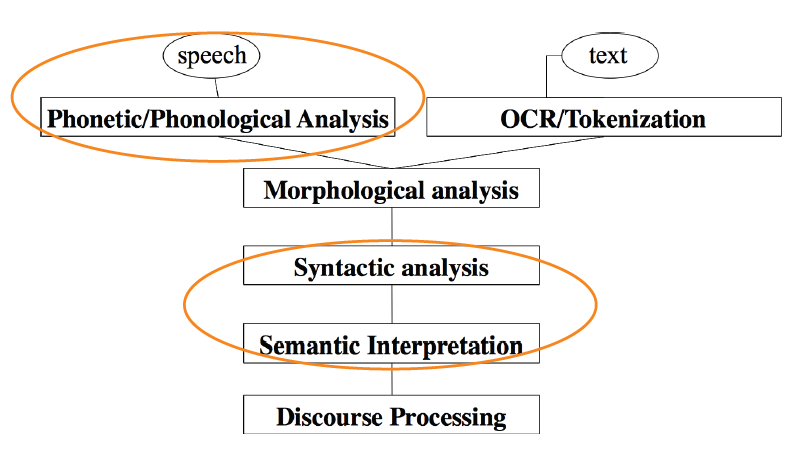
\includegraphics[scale=0.3]{nlp_level}
\caption{NLP Level}
\end{figure}


\end{document}